%%%%%%%%%%%%%%%%%%%%%%%%%%%%%%%%%%%%%%%%%%%%%%%%%%%%%%%%%%%%%%%%%%%%%%%%%%%%%%%%%%
\begin{frame}[fragile]\frametitle{}
\begin{center}
{\Large Database}
\end{center}
\end{frame}

%%%%%%%%%%%%%%%%%%%%%%%%%%%%%%%%%%%%%%%%%%%%%%%%%%%%%%%%%%%%%%%%%%%%%%%%%%%%%%%%%%
\begin{frame}\frametitle{A Brief DB History}

Early 1970s

\begin{itemize}
\item Many database systems
\item Incompatible, exposing many implementation details
\end{itemize}

Then Ted Codd came along
\begin{itemize}
\item Relational model
\item Structured Query Language (SQL)
\item Implementation differences became irrelevant
\item A few major DB systems dominated the market
\end{itemize}


{\tiny (Ref: Are Relational Databases the Only Type of Databases? )}
\end{frame}


%%%%%%%%%%%%%%%%%%%%%%%%%%%%%%%%%%%%%%%%%%%%%%%%%%%%%%%%%%%%%%%%%%%%%%%%%%%%%%%%%%
\begin{frame}\frametitle{Architecture Changes Over Time }
1980’s: Single Application


\begin{center}
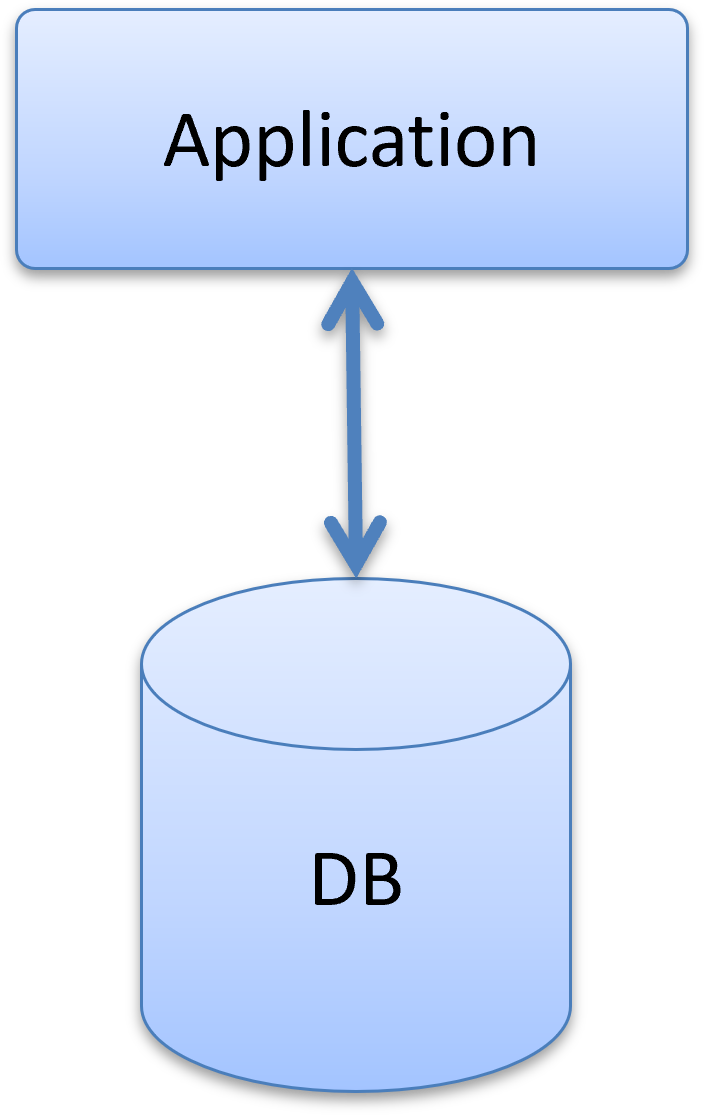
\includegraphics[width=0.4\linewidth,keepaspectratio]{neo4j52}
\end{center}	

{\tiny (Ref: NoSQL: Graph Databases)}

\end{frame}

%%%%%%%%%%%%%%%%%%%%%%%%%%%%%%%%%%%%%%%%%%%%%%%%%%%%%%%%%%%%%%%%%%%%%%%%%%%%%%%%%%
\begin{frame}\frametitle{Architecture Changes Over Time }
Database Antipattern


\begin{center}
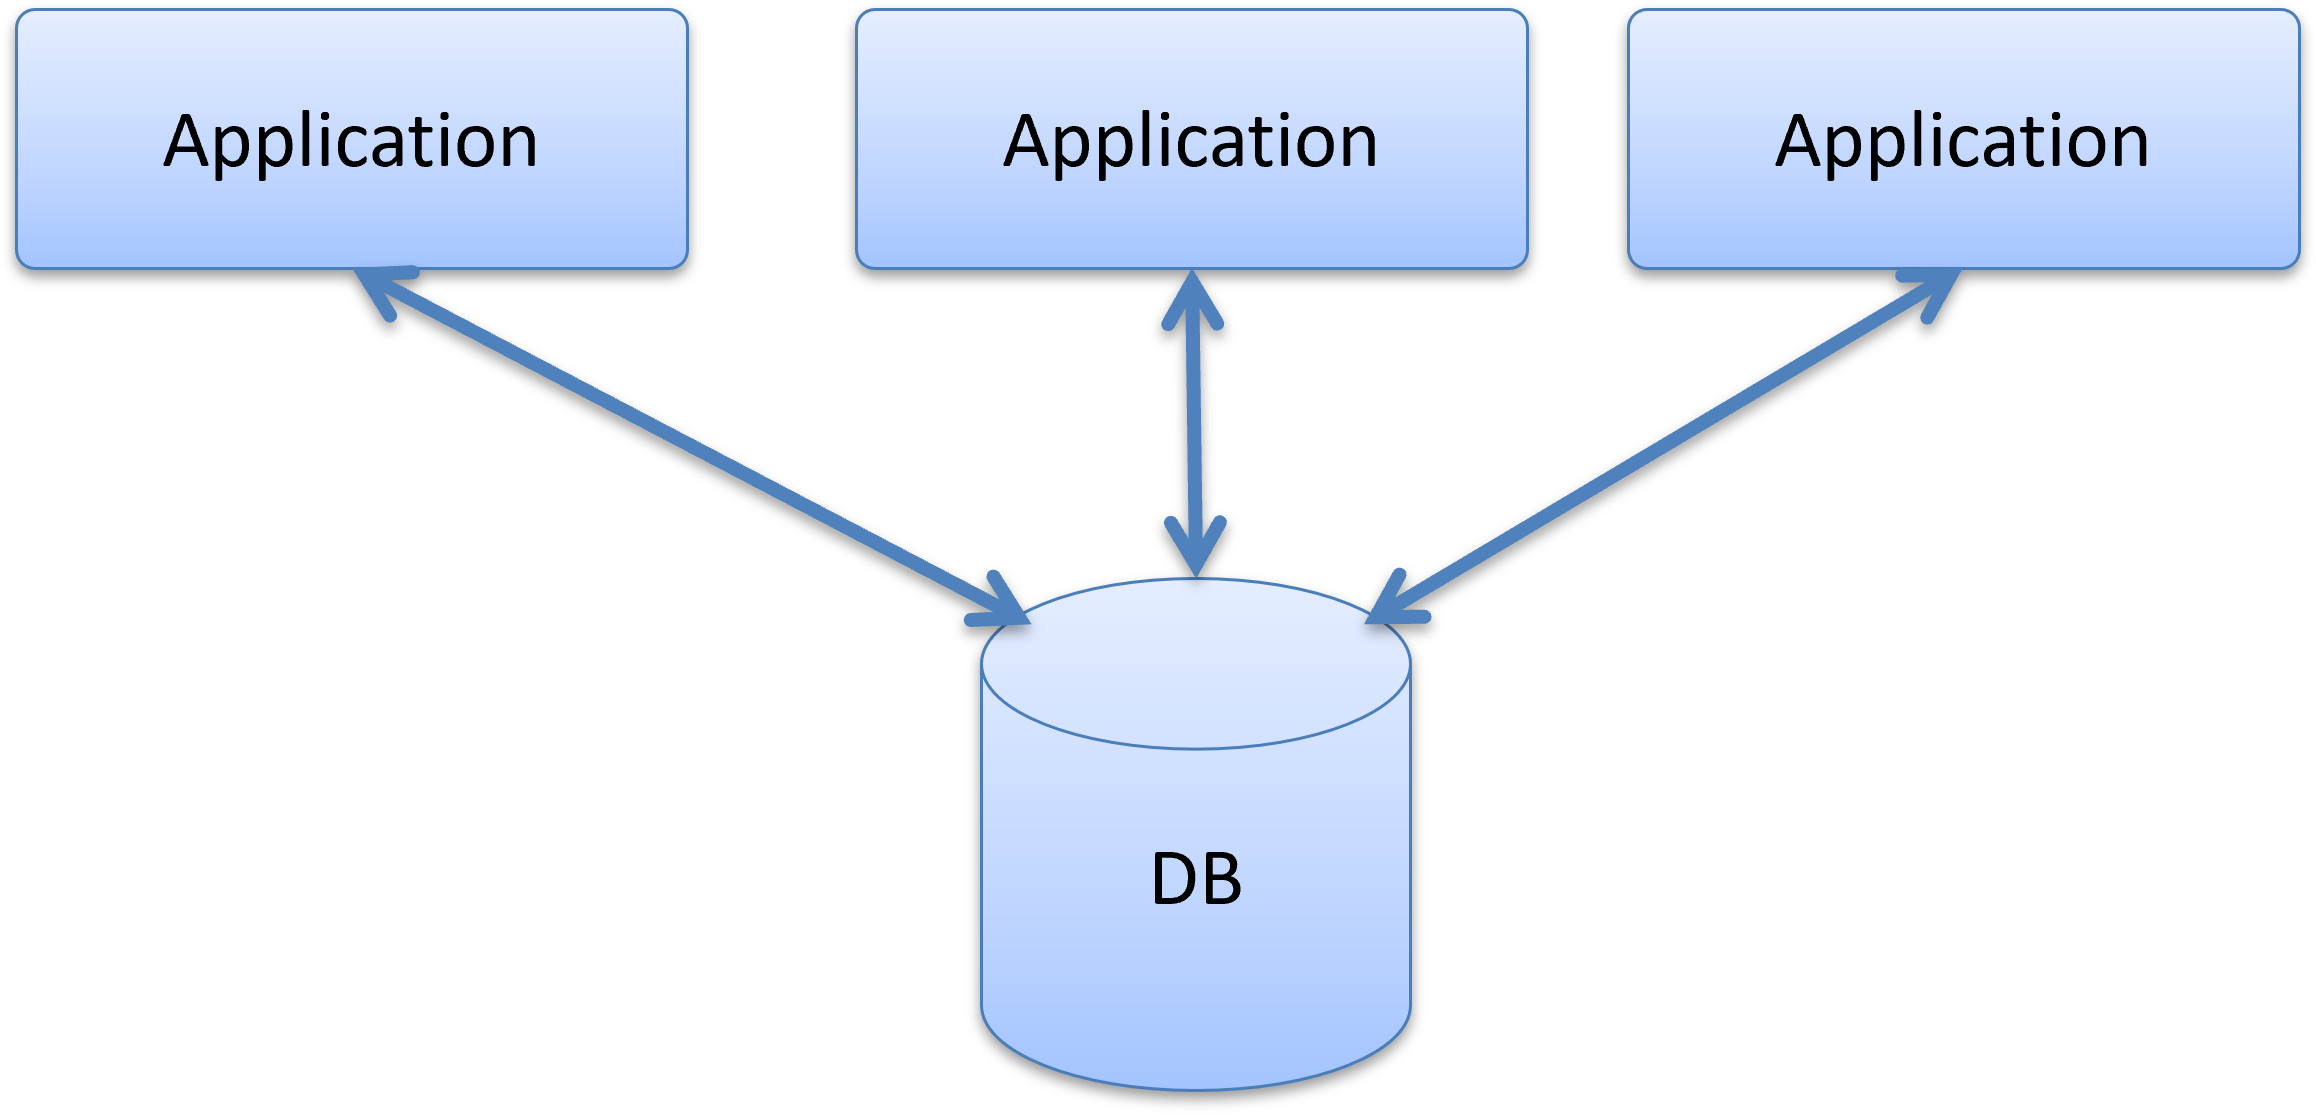
\includegraphics[width=0.4\linewidth,keepaspectratio]{neo4j53}
\end{center}	

{\tiny (Ref: NoSQL: Graph Databases)}

\end{frame}


%%%%%%%%%%%%%%%%%%%%%%%%%%%%%%%%%%%%%%%%%%%%%%%%%%%%%%%%%%%%%%%%%%%%%%%%%%%%%%%%%%
\begin{frame}\frametitle{Architecture Changes Over Time }
2000’s: SOA



\begin{center}
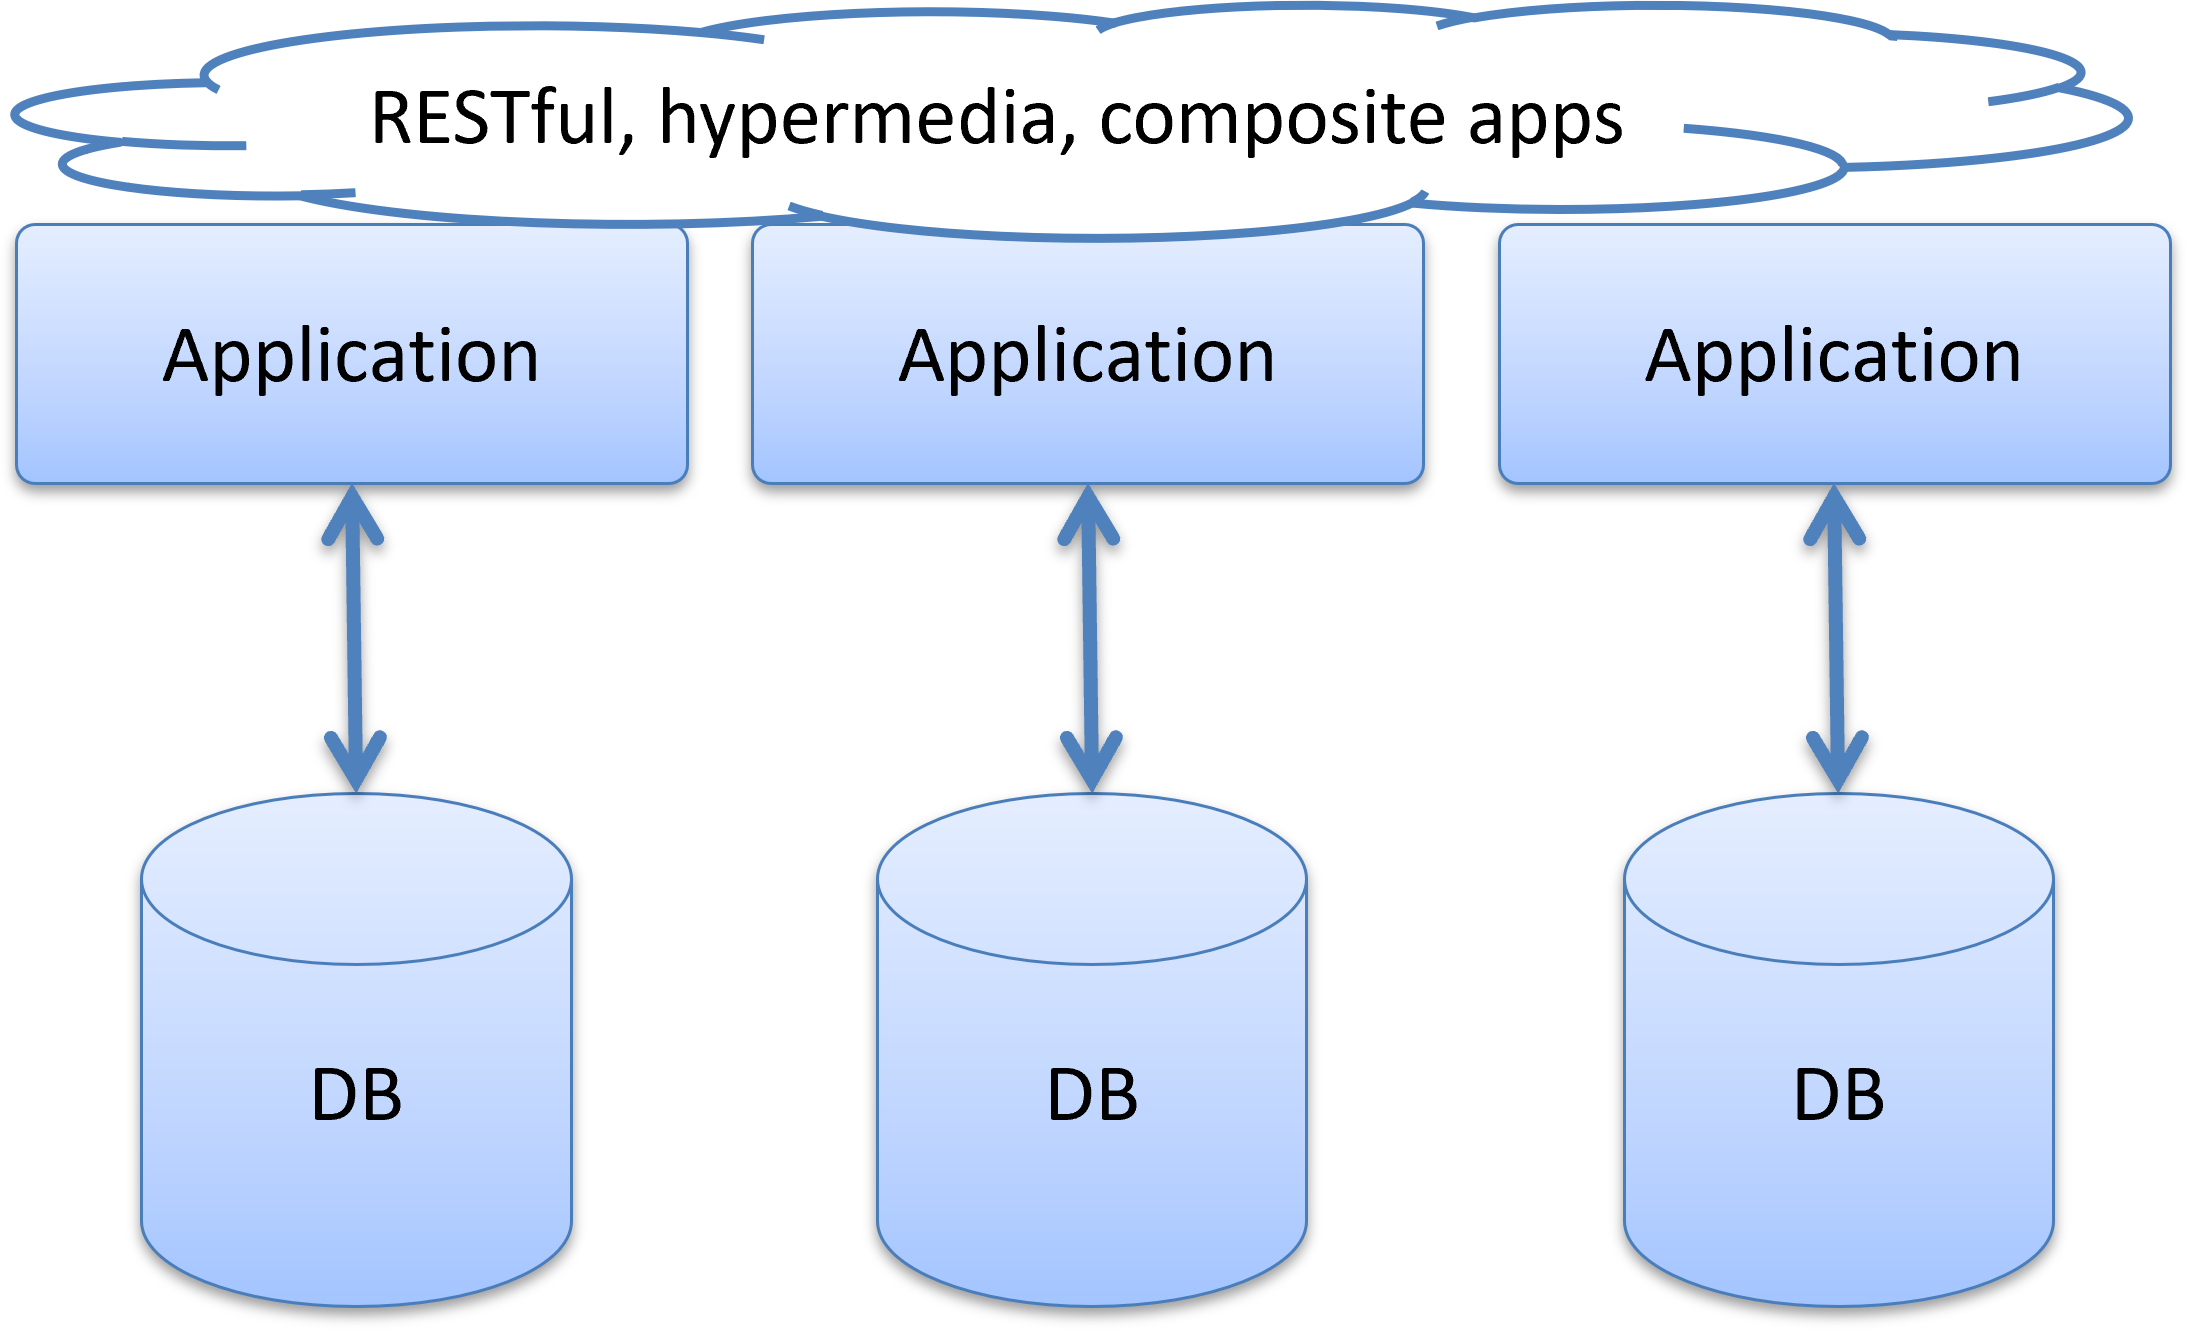
\includegraphics[width=0.4\linewidth,keepaspectratio]{neo4j54}
\end{center}	

{\tiny (Ref: NoSQL: Graph Databases)}

\end{frame}


%%%%%%%%%%%%%%%%%%%%%%%%%%%%%%%%%%%%%%%%%%%%%%%%%%%%%%%%%%%%%%%%%%%%%%%%%%%%%%%%%%
\begin{frame}\frametitle{Web 1/2/3 and Big Data}


\begin{itemize}
\item Twitter: 350 million monthly active users and 500 million Tweets are sent per day,
\item Facebook: over 1 billion monthly users and faces 3 million message per 20 minute
\item Instagram: 200 Million Monthly Active Users and 1.6 Billion Likes and 60 Million Photos shared every day

\end{itemize}


{\tiny (Ref: Are Relational Databases the Only Type of Databases? )}
\end{frame}


%%%%%%%%%%%%%%%%%%%%%%%%%%%%%%%%%%%%%%%%%%%%%%%%%%%%%%%%%%%%%%%%%%%%%%%%%%%%%%%%%%
\begin{frame}\frametitle{Background}

Data is more connected:

\begin{itemize}
\item Text (content)
\item  HyperText (added pointers)
\item  RSS (joined those pointers)
\item Blogs (added pingbacks)
\item Tagging (grouped related data)
\item RDF (described connected data)
\item GGG (content + pointers + relationships + descriptions)
\end{itemize}

 

{\tiny (Ref: CIntroduction to Graph Databases - Max De Marzi )}
\end{frame}

%%%%%%%%%%%%%%%%%%%%%%%%%%%%%%%%%%%%%%%%%%%%%%%%%%%%%%%%%%%%%%%%%%%%%%%%%%%%%%%%%%
\begin{frame}\frametitle{Structured Unstructured}


\begin{center}
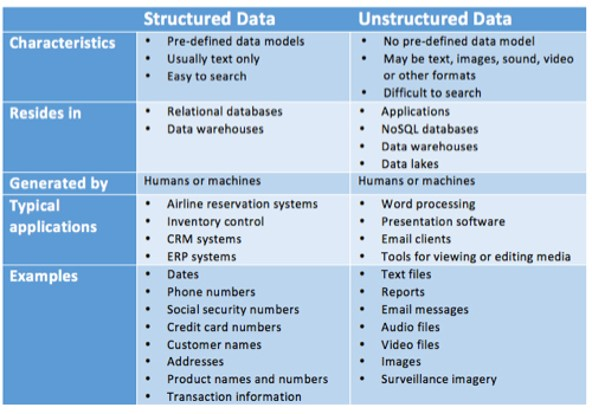
\includegraphics[width=0.5\linewidth,keepaspectratio]{neo4j49}
\end{center}	

{\tiny (Ref: https://www.datamation.com/big-data/structured-vs-unstructured-data.html)}
\end{frame}

%%%%%%%%%%%%%%%%%%%%%%%%%%%%%%%%%%%%%%%%%%%%%%%%%%%%%%%%%%%%%%%%%%%%%%%%%%%%%%%%%%
\begin{frame}\frametitle{Database Systems Landscape }


\begin{center}
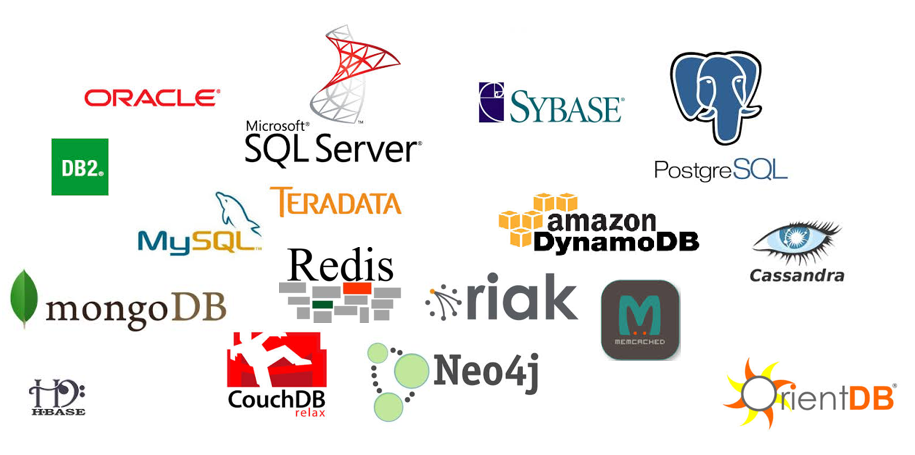
\includegraphics[width=\linewidth,keepaspectratio]{neo4j50}
\end{center}	

{\tiny (Ref: Are Relational Databases the Only Type of Databases? )}

\end{frame}



%%%%%%%%%%%%%%%%%%%%%%%%%%%%%%%%%%%%%%%%%%%%%%%%%%%%%%%%%%%%%%%%%%%%%%%%%%%%%%%%%%
\begin{frame}\frametitle{Introduction}

\begin{itemize}
\item A Database is a place to store application data, to process and query, etc

\item Relational databases (SQL) store data in tables. Strict schema.
\item Document Db: key-value databases (no-SQL) store data in dictionaries/json. Flexi schema.
\item A Graph Database is where data is stored in graph data structure ie nodes and edges.
\end{itemize}

\begin{center}
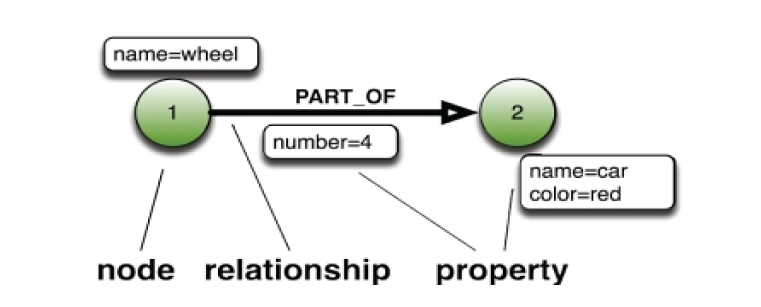
\includegraphics[width=0.5\linewidth,keepaspectratio]{neo4j29}
\end{center}	

{\tiny (Ref: Neo4j (Graph Database) Crash Course - Laith Academy)}
\end{frame}


%%%%%%%%%%%%%%%%%%%%%%%%%%%%%%%%%%%%%%%%%%%%%%%%%%%%%%%%%%%%%%%%%%%%%%%%%%%%%%%%%%
\begin{frame}\frametitle{Database Systems Landscape }


\begin{center}
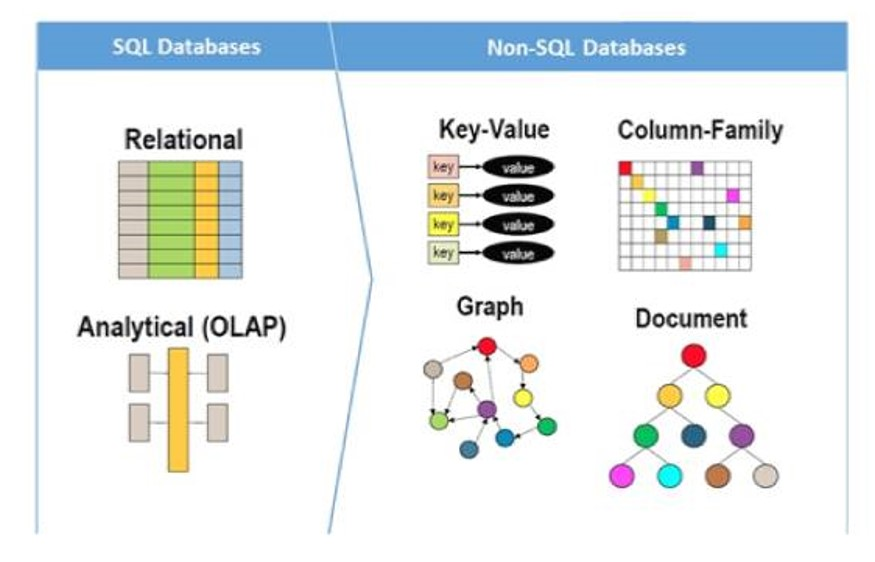
\includegraphics[width=\linewidth,keepaspectratio]{neo4j51}
\end{center}	

{\tiny (Ref: Are Relational Databases the Only Type of Databases? )}

\end{frame}


%%%%%%%%%%%%%%%%%%%%%%%%%%%%%%%%%%%%%%%%%%%%%%%%%%%%%%%%%%%%%%%%%%%%%%%%%%%%%%%%%%
\begin{frame}\frametitle{What is a Graph Database?}

\begin{itemize}
\item A database with an explicit graph structure
\item Each node knows its adjacent nodes 
\item As the number of nodes increases, the cost of a local step (or hop) remains the same
\item Plus an Index for lookups
\end{itemize}

{\tiny (Ref: CIntroduction to Graph Databases - Max De Marzi )}
\end{frame}


%%%%%%%%%%%%%%%%%%%%%%%%%%%%%%%%%%%%%%%%%%%%%%%%%%%%%%%%%%%%%%%%%%%%%%%%%%%%%%%%%%
\begin{frame}\frametitle{Example}


\begin{center}
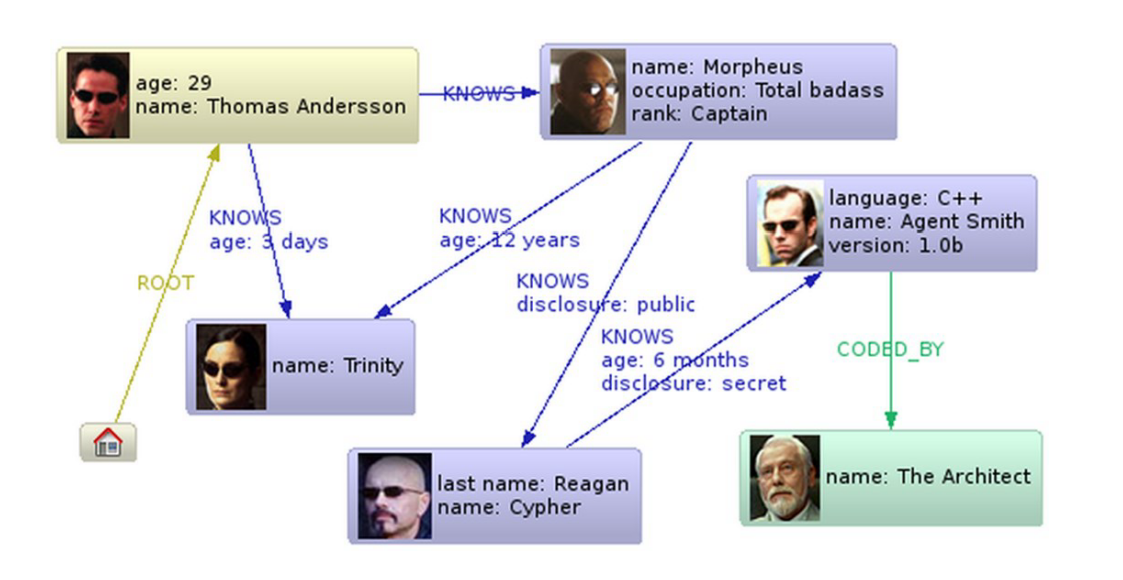
\includegraphics[width=\linewidth,keepaspectratio]{neo4j30}
\end{center}	

{\tiny (Ref: CIS 6930 - Advanced Databases - Neo4j )}
\end{frame}

%%%%%%%%%%%%%%%%%%%%%%%%%%%%%%%%%%%%%%%%%%%%%%%%%%%%%%%%%%%
\begin{frame}[fragile]\frametitle{Relational Database}
SQL

\begin{center}
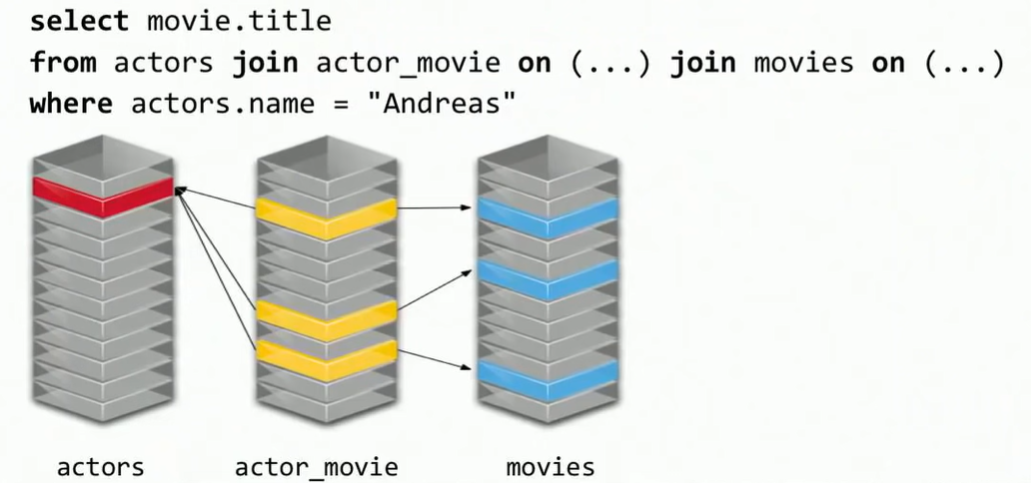
\includegraphics[width=\linewidth,keepaspectratio]{neo4j17}
\end{center}	    

{\tiny (Ref: Introduction to Neo4j and Graph Databases
 - M David Allen)}

\end{frame}

%%%%%%%%%%%%%%%%%%%%%%%%%%%%%%%%%%%%%%%%%%%%%%%%%%%%%%%%%%%
\begin{frame}[fragile]\frametitle{Graph Database}
Cypher

\begin{center}
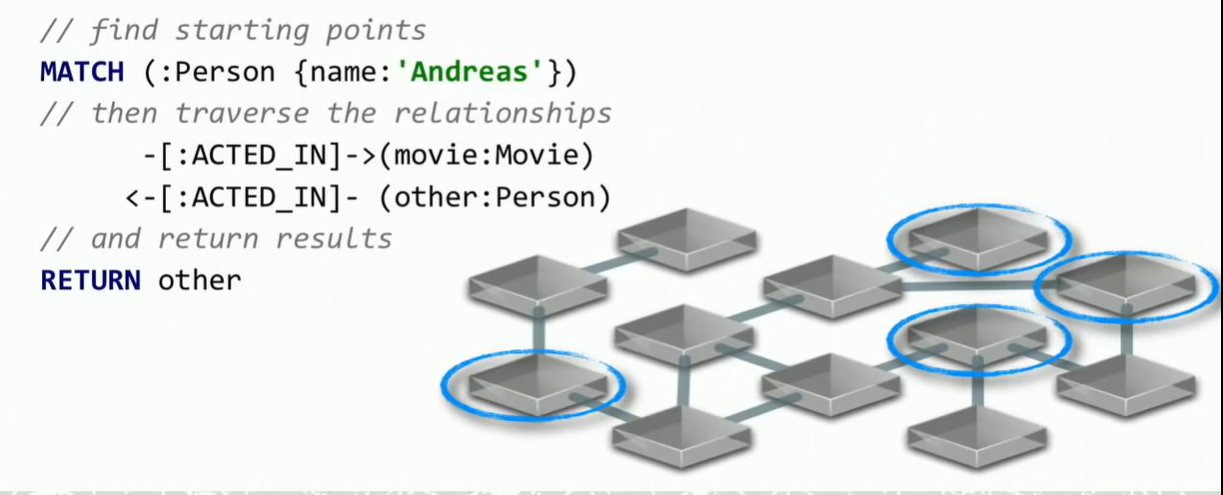
\includegraphics[width=\linewidth,keepaspectratio]{neo4j18}
\end{center}	    

{\tiny (Ref: Introduction to Neo4j and Graph Databases
 - M David Allen)}

\end{frame}

%%%%%%%%%%%%%%%%%%%%%%%%%%%%%%%%%%%%%%%%%%%%%%%%%%%%%%%%%%%%%%%%%%%%%%%%%%%%%%%%%%
\begin{frame}\frametitle{RDBMS}

\begin{itemize}
\item Cannot model or store data and relationships well, ie, without complexity
\item Performance degrades with umber and levels of relationships and database size
\item Query complexity grows with the need for JOINs
\item Adding new types of data and relationships requires schema redesign
\item More difficult if that needs to be done real time.
\end{itemize}

{\tiny (Ref: Neo4j (Graph Database) Crash Course - Laith Academy)}
\end{frame}

%%%%%%%%%%%%%%%%%%%%%%%%%%%%%%%%%%%%%%%%%%%%%%%%%%%%%%%%%%%%%%%%%%%%%%%%%%%%%%%%%%
\begin{frame}\frametitle{Comparing RDBMS to Graph database}

\begin{center}
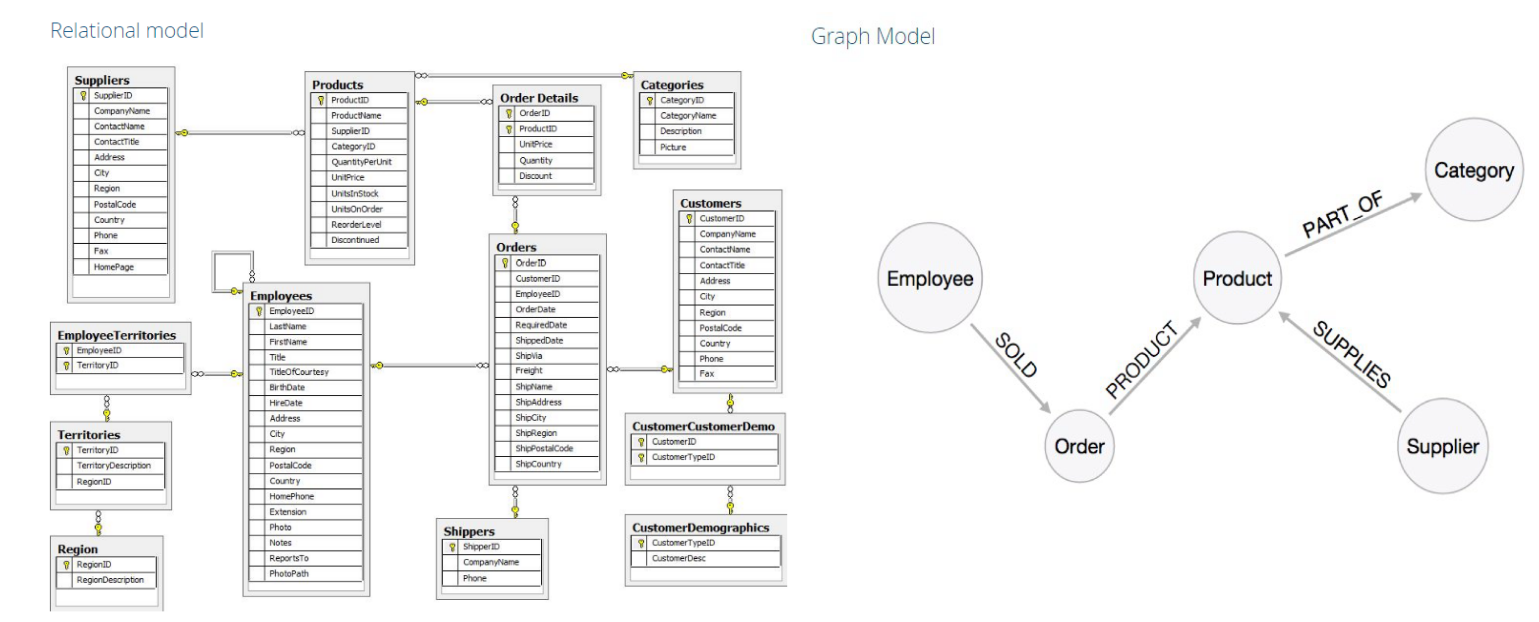
\includegraphics[width=\linewidth,keepaspectratio]{neo4j39}
\end{center}	  


{\tiny (Ref: CIS 6930 - Advanced Databases - Neo4j )}
\end{frame}

%%%%%%%%%%%%%%%%%%%%%%%%%%%%%%%%%%%%%%%%%%%%%%%%%%%%%%%%%%%%%%%%%%%%%%%%%%%%%%%%%%
\begin{frame}\frametitle{Comparing RDBMS to Graph database}

\begin{center}
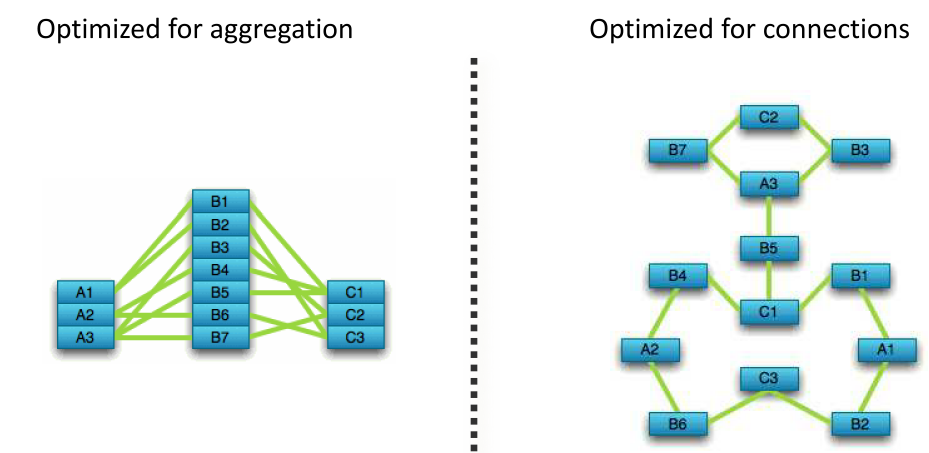
\includegraphics[width=\linewidth,keepaspectratio]{neo4j43}
\end{center}	  


{\tiny (Ref: CIntroduction to Graph Databases - Max De Marzi )}
\end{frame}

%%%%%%%%%%%%%%%%%%%%%%%%%%%%%%%%%%%%%%%%%%%%%%%%%%%%%%%%%%%%%%%%%%%%%%%%%%%%%%%%%%
\begin{frame}\frametitle{Comparing Key Value Stores to Graph database}

\begin{center}
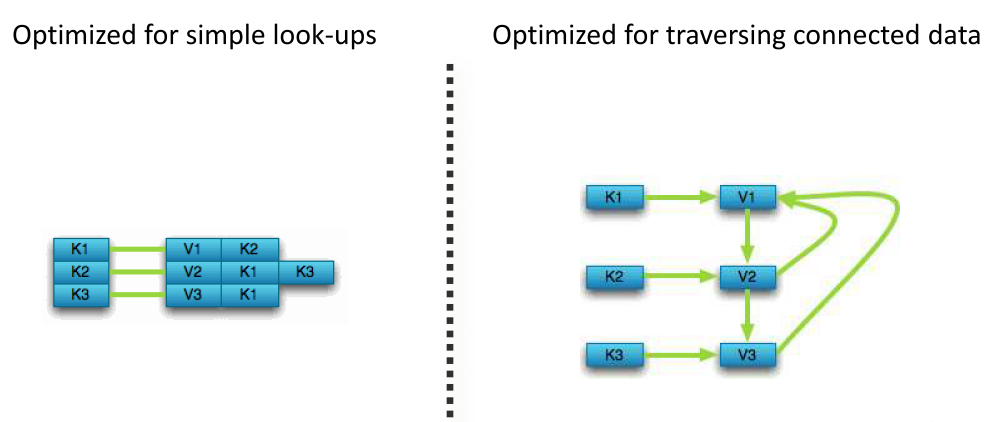
\includegraphics[width=\linewidth,keepaspectratio]{neo4j44}
\end{center}	  


{\tiny (Ref: CIntroduction to Graph Databases - Max De Marzi )}
\end{frame}

%%%%%%%%%%%%%%%%%%%%%%%%%%%%%%%%%%%%%%%%%%%%%%%%%%%%%%%%%%%%%%%%%%%%%%%%%%%%%%%%%%
\begin{frame}\frametitle{Comparing Key Value Stores to Graph database}

\begin{center}
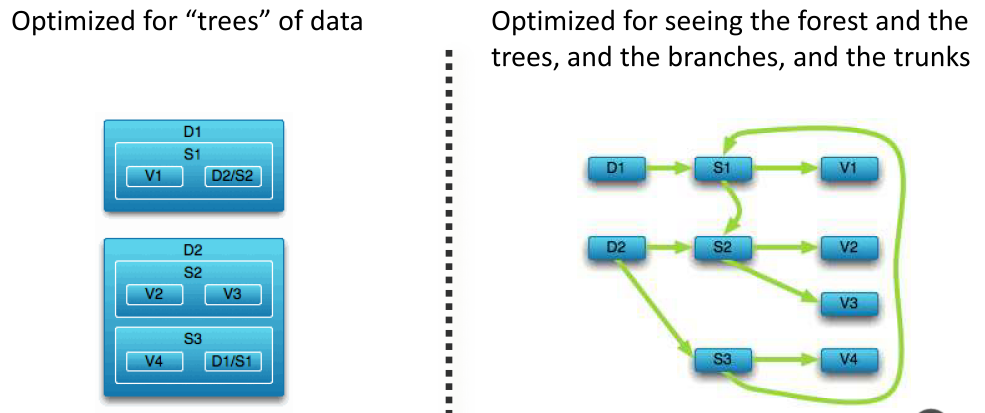
\includegraphics[width=\linewidth,keepaspectratio]{neo4j45}
\end{center}	  


{\tiny (Ref: CIntroduction to Graph Databases - Max De Marzi )}
\end{frame}




% %%%%%%%%%%%%%%%%%%%%%%%%%%%%%%%%%%%%%%%%%%%%%%%%%%%%%%%%%%%%%%%%%%%%%%%%%%%%%%%%%%
% \begin{frame}\frametitle{Comparing the Joins and Cypher Query}

% We want to see who bought Chocolade. Let’s join the four tables together in Relational Model


% \begin{lstlisting}
% SELECT DISTINCT c.CompanyName
% FROM customers AS c
% JOIN orders AS o ON (c.CustomerID = o.CustomerID)
% JOIN order_details AS od ON (o.OrderID = od.OrderID)
% JOIN products AS p ON (od.ProductID = p.ProductID)
% WHERE p.ProductName = 'Chocolade';
% \end{lstlisting}	  

% The graph model is much simpler, as we don’t need join tables, and expressing connections as graph patterns, is easier to read too.

% \begin{lstlisting}
% MATCH (p:Product {productName:"Chocolade"})<-[:PRODUCT]-(:Order)<-[:PURCHASED]-(c:Customer)
% RETURN distinct c.companyName;
% \end{lstlisting}	  


% {\tiny (Ref: CIS 6930 - Advanced Databases - Neo4j )}
% \end{frame}


%%%%%%%%%%%%%%%%%%%%%%%%%%%%%%%%%%%%%%%%%%%%%%%%%%%%%%%%%%%
\begin{frame}[fragile]\frametitle{Comparison}
Find all reports and how many people they manage upto 3 levels down.

\begin{center}
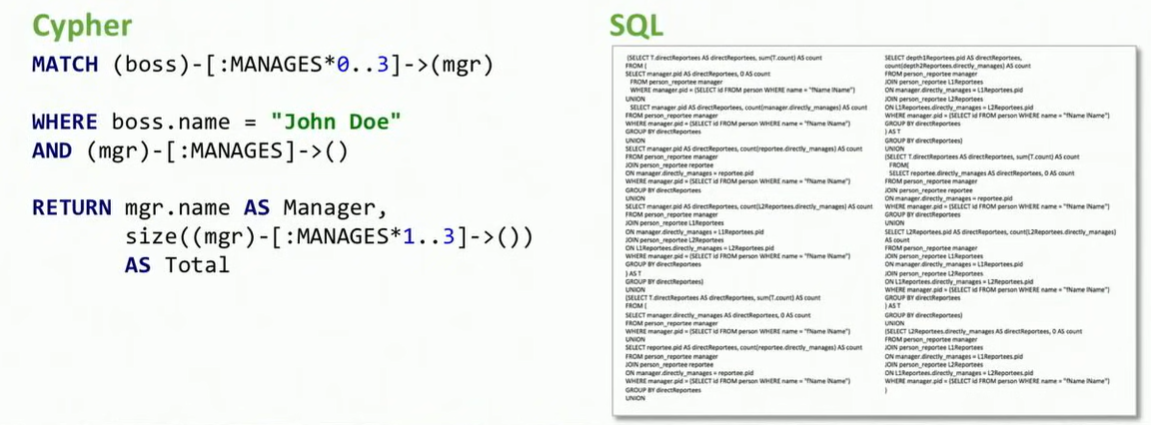
\includegraphics[width=\linewidth,keepaspectratio]{neo4j19}
\end{center}	    

{\tiny (Ref: Introduction to Neo4j and Graph Databases
 - M David Allen)}

\end{frame}

%%%%%%%%%%%%%%%%%%%%%%%%%%%%%%%%%%%%%%%%%%%%%%%%%%%%%%%%%%%
\begin{frame}[fragile]\frametitle{Same Data, Different Layout}
No more Tables, no more Doreign Keys, no more Joins
\begin{center}
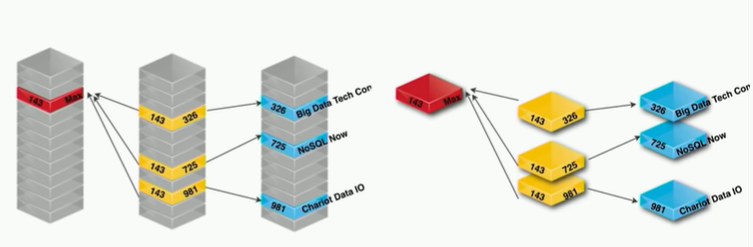
\includegraphics[width=\linewidth,keepaspectratio]{neo4j22}
\end{center}	    

{\tiny (Ref: Secret Sauce of Neo4j: Modeling and Querying Graphs
 - Max De Marzi )}

\end{frame}

%%%%%%%%%%%%%%%%%%%%%%%%%%%%%%%%%%%%%%%%%%%%%%%%%%%%%%%%%%%
\begin{frame}[fragile]\frametitle{Relational Databases cannot do Relationships}

\begin{center}
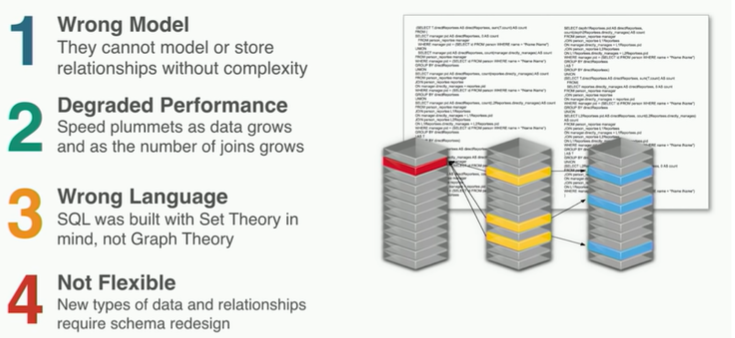
\includegraphics[width=\linewidth,keepaspectratio]{neo4j23}
\end{center}	    

{\tiny (Ref: Secret Sauce of Neo4j: Modeling and Querying Graphs
 - Max De Marzi )}

\end{frame}

%%%%%%%%%%%%%%%%%%%%%%%%%%%%%%%%%%%%%%%%%%%%%%%%%%%%%%%%%%%
\begin{frame}[fragile]\frametitle{No-SQL Databases cannot do Relationships}
Key-value pairs, no Joins, no connections

\begin{center}
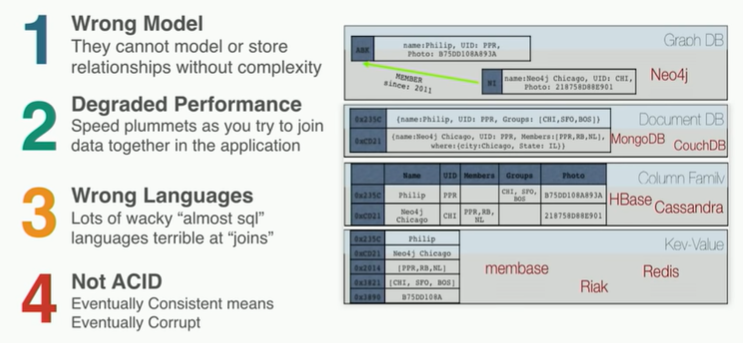
\includegraphics[width=\linewidth,keepaspectratio]{neo4j24}
\end{center}	    

{\tiny (Ref: Secret Sauce of Neo4j: Modeling and Querying Graphs
 - Max De Marzi )}

\end{frame}




%%%%%%%%%%%%%%%%%%%%%%%%%%%%%%%%%%%%%%%%%%%%%%%%%%%%%%%%%%%
\begin{frame}[fragile]\frametitle{Performance}
Remains steady as Database grows. Btw, suitable for graph like data only, and not like lists-queues like dataset where RDBM will work far better.

\begin{center}
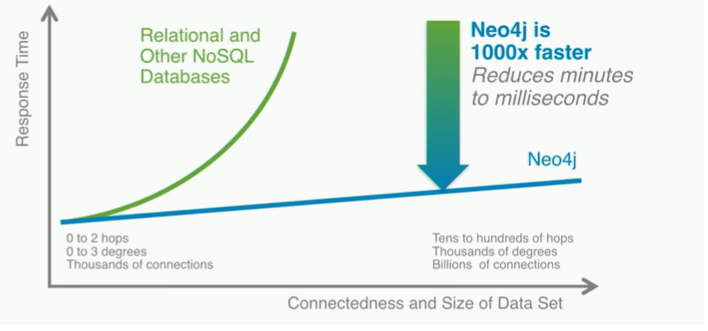
\includegraphics[width=\linewidth,keepaspectratio]{neo4j25}
\end{center}	    

{\tiny (Ref: Secret Sauce of Neo4j: Modeling and Querying Graphs
 - Max De Marzi )}

\end{frame}

%%%%%%%%%%%%%%%%%%%%%%%%%%%%%%%%%%%%%%%%%%%%%%%%%%%%%%%%%%%
\begin{frame}[fragile]\frametitle{Smells like a Graph?}

\begin{center}
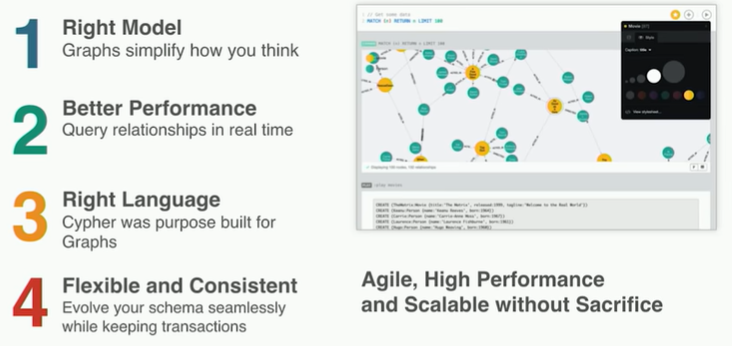
\includegraphics[width=\linewidth,keepaspectratio]{neo4j26}
\end{center}	    

{\tiny (Ref: Secret Sauce of Neo4j: Modeling and Querying Graphs
 - Max De Marzi )}

\end{frame}

%%%%%%%%%%%%%%%%%%%%%%%%%%%%%%%%%%%%%%%%%%%%%%%%%%%%%%%%%%%%%%%%%%%%%%%%%%%%%%%%%%
\begin{frame}\frametitle{Use Cases}


\begin{itemize}
\item  Real time recommendation
\item  Master data management 
\item  Fraud detection
\item  Graph based search 
\item  IT operations and network management 
\end{itemize}


{\tiny (Ref: CIS 6930 - Advanced Databases - Neo4j )}
\end{frame}

%%%%%%%%%%%%%%%%%%%%%%%%%%%%%%%%%%%%%%%%%%%%%%%%%%%%%%%%%%%%%%%%%%%%%%%%%%%%%%%%%%
\begin{frame}\frametitle{Successful companies using graphs}


\begin{center}
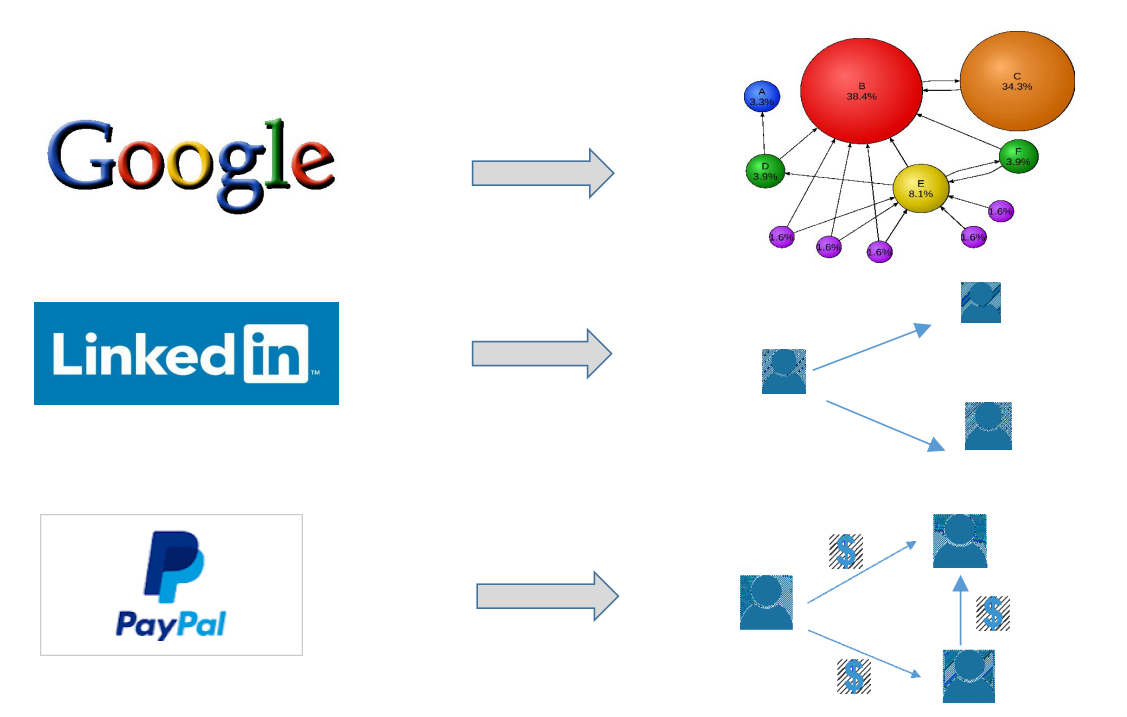
\includegraphics[width=0.8\linewidth,keepaspectratio]{neo4j31}
\end{center}	

{\tiny (Ref: CIS 6930 - Advanced Databases - Neo4j )}
\end{frame}

